\section{Methodology}\label{sec-methodology}

This study adopts a quasi-experimental research design, employing a
pre-established group comprising preservice foreign language teachers
who met the requisite criteria for participation. The research was
conducted in a field setting over the course of a three-hour session.
Initially, the teacher trainer provided an overview of the TWEE tool,
after which participants engaged with it to develop teaching materials
for foreign language instruction. Subsequently, participants completed a
questionnaire designed to gather both qualitative and quantitative data,
following their practical introduction to the tool during the class
session.

The SWOT analysis, developed by \textcite{learned1965} in the 1960s, is a
strategic planning tool that has found widespread utility in evaluating
projects or organizations, transcending its original context in business
planning \cite{chermack2007} to become applicable in academic
evaluation research \cite{romerogutierrez2015}. The acronym SWOT
represents Strengths, Weaknesses, Opportunities, and Threats, and it is
interchangeably known as TOWS analysis. This analytical approach is
designed to provide a holistic assessment of both internal elements,
including strengths and weaknesses, and external factors, comprising
opportunities and threats. The data analysis included content analysis
of qualitative data to categorizing and arranging them into the SWOT
matrix. Content analysis is ``as a systematic, replicable technique for
compressing many words of text into fewer content categories based on
explicit rules of coding'' \cite{stemler2000}. The systematic exploration
of these internal and external dimensions allows for a comprehensive
understanding of the positive and negative aspects of a project or tool.
In the context of analyzing the use of TWEE for language teaching, the
SWOT analysis proves invaluable. It enables educators and stakeholders
to identify the internal strengths, such as enhancing personalized
learning, and weaknesses, like potential biases in AI algorithms.
Simultaneously, it helps in recognizing external opportunities, such as
improved language learning outcomes, and threats, such as ethical
concerns and potential misuse of TWEE. Through this analytical
framework, a systematic examination can inform strategic planning,
ensuring the maximization of positive outcomes while addressing and
mitigating potential challenges in integrating TWEE into language
teaching practices (\Cref{img-01}).

\begin{figure}[!htbp]
    \centering
    \caption{2x2 Matrix for SWOT Analysis.}
    \label{img-01}
    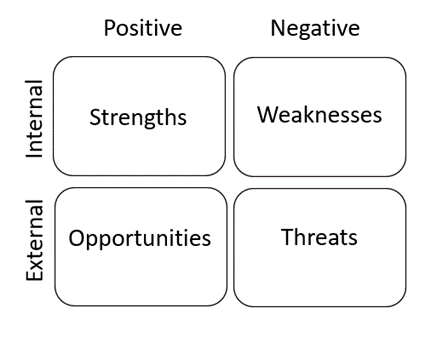
\includegraphics[width=0.5\textwidth]{image1.png}
    \source{Adapted from \textcite[p. 387]{chermack2007}}
\end{figure}

\subsection{TWEE: A.I. Powered Tools For English Teachers}\label{sub-sec-twee}

TWEE, as delineated by \textcite{ravshanovna2023}, represents an AI-driven
instrument facilitating the creation of educational tasks tailored to
EFL and ESL courses. Through the provision of various prompts
encompassing language proficiency, topic, and word count, among others,
TWEE generates activities targeting different linguistic skills such as
reading, writing, listening, and speaking, alongside grammar and
vocabulary exercises. It generates activities after providing several
prompts (e.g. language level, topic, number of words, etc.) of the
different linguistic skills (reading, writing, listening and speaking)
as well as grammar and vocabulary activities, hence, reducing teachers'
material preparation time. Activities such as word formation, Youtube
video exercises, speaking prompts, creative writing and T/F questions
are some of the examples this tool may generate for the English language
teacher This functionality significantly diminishes the time spent by
instructors on material preparation. Among the array of activities TWEE
can generate are word formation tasks, YouTube video exercises, speaking
prompts, creative writing tasks, and True/False questions, thereby
catering to diverse pedagogical needs.

Furthermore, \textcite[p.~101]{delarosa2023} expounds on the transformative
impact of AI tools like ChatGPT and TWEE on time management in language
instruction. The conventional paradigm of teachers expending substantial
time on planning, exercise creation, and content generation has shifted
towards a more efficient utilization of time resources. With the
integration of AI-based solutions, such as TWEE, these tasks are
streamlined, affording educators the opportunity to redirect their focus
towards teaching. De la Rosa also highlights alternative AI tools like
Gamma ai and Diffit for teachers ai, which offer functionalities akin to
ChatGPT and TWEE in generating customized content. Notably, TWEE stands
out due to its ability to generate various language learning activities,
including fill-in-the-gap exercises, word formation tasks, YouTube video
exercises, and summaries, aligning with the requisites of standardized
English language assessments.

\subsection{Participants}\label{sub-sec-participants}

The participants in this study comprised 29 pre-service secondary school
teachers undertaking the Master's Degree in Secondary Education.
Questions 1 through 6 of the questionnaire aimed at profiling them
concerning both their training and teaching experience. The participants
exhibited a diverse array of university degrees, with the majority
holding degrees in English Philology (82\%) and translation and
interpreting (14\%). They possess the capacity to instruct English
(63\%) and other languages, including French (13\%), Portuguese (6\%),
and German (3\%) in certain cases. In terms of age demographics, a
significant proportion of participants fell within the range of 20 to 25
years (73\%), while a smaller subset spanned from 26 to 30 (14\%) and 31
to 35 (14\%) years old. Notably, 55\% of the participants have prior
teaching experience in foreign languages, predominantly in private or
academic settings, encompassing a spectrum of proficiency levels from
elementary to advanced (A1, B1, C1).

\subsection{Research tool}\label{sub-sec-researchtool}

The formulation of the specific questionnaire emanated from the
adaptation of instruments utilized by \textcite{fernandezcostales2021}. Employing the Delphi technique, characterized as a
communication structure designed to facilitate a thorough critical
examination and discourse \cite{green2014}, the initial questionnaire
underwent assessment by three researchers specializing in foreign
language teaching and three practitioners in secondary language
education. This iterative process aimed to elicit their perspectives and
pinpoint pivotal topics for discussion. Subsequently, the insights
proffered by the experts were incorporated into the final questionnaire,
which encompassed three distinct sections.

The first section was devised to profile the participants, encompassing
their language teaching training, experiences, general perceptions, and
use of AI for general purposes. This profiling aimed to pre-establish
potential implications for their subsequent responses in the ensuing
questions. The second segment exclusively concentrated on identifying
the internal strengths and weaknesses of the AI tool TWEE, along with
the external opportunities and threats associated with its
implementation in secondary education settings. The third and final
section of the questionnaire gathered information on prospective
teachers' perceptions of AI for general teaching
purposes.

\subsection{Data analysis}\label{sub-sec-dataanalysis}
\subsubsection{Participants use of Artificial Intelligence}\label{sub-sub-sec-participantsuseof}

In terms of their engagement with AI for academic purposes, the data
indicates a diverse spectrum of utilization among participants (see
\Cref{table-01}). While some explicitly state a lack of utilization of AI tools
for academic tasks, others detail specific platforms such as ChatGPT,
DeepL, Reverso, and Bing Image Generator. Notably, the reasons behind
tool usage vary significantly. For instance, some participants employ
ChatGPT primarily for idea generation and structuring, while others
utilize it for initial brainstorming sessions. DeepL emerges as a
popular choice for translation tasks, particularly in instances where
composition poses challenges. Furthermore, participants often integrate
multiple AI tools, such as ChatGPT and DeepL, suggesting a complementary
approach to leveraging various platforms for academic enhancement.
Additionally, the inclusion of tools like Canva and WordReference
alongside AI tools reflects a comprehensive approach to academic tasks,
encompassing a variety of resources to optimize both productivity and
quality. Overall, the data illustrates a broad array of preferences and
strategies in utilizing AI tools for academic pursuits, highlighting the
flexibility and adaptability of these technologies in supporting
scholarly endeavors.

Regarding the participants' utilization of AI tools for
teaching and learning foreign languages, the data reveals a diverse set
of approaches and preferences. While some participants report no use of
AI tools for this purpose, others mention specific platforms like
ChatGPT, DeepL, Reverso, and Bing Image Generator. Notably, there is an
indication of an openness to explore new tools, such as TWEE, suggesting
a willingness to embrace innovative technologies for language
instruction in the near future. Furthermore, participants often employ
combinations of tools such as Paddlet, Duolingo, and ChatGPT, indicating
a multifaceted approach to language teaching and learning. ChatGPT
emerges as a versatile tool, utilized for generating ideas for class
dynamics, exercises, and other instructional materials. Moreover,
participants integrate AI tools with other resources like Canva and Bing
Image Generator, showcasing a holistic approach to language education
that incorporates various technological and creative elements. Overall,
the data underscores the varied strategies employed by participants in
leveraging AI tools to enhance the teaching and learning experience in
foreign language education. Most of these tools can be categorized
following \posscite{baker2019} AI-powered language learning tools
scenarios.

Regarding the use of AI for translation activities, the data showcases a
variety of preferences and approaches. While some participants do not
use any AI tools for translation purposes, others specifically mention
platforms such as DeepL, Reverso, Cambridge Dictionary, and Google
Translate. Notably, there is a mention of a participant preferring
direct consultation of a dictionary, indicating a preference for
traditional reference materials over AI-powered translation tools for
learning assistance. DeepL emerges as a prominent choice among
participants, often combined with other resources like WordReference and
Reverso for comprehensive translation tasks. Additionally, participants
highlight DeepL's accuracy and reliability, underscoring
its effectiveness in facilitating translation activities. Overall, the
data reflects a range of strategies employed by participants in
leveraging AI tools for translation, with DeepL being prevalent due to
its robust functionality and versatility in assisting with linguistic
tasks. These translation tools are also being used successfully for
language learning purposes \cite{birdsell2022,cotellikureth2023}.

In terms of other uses of AI, the data highlights the diverse
applications and functionalities of AI tools beyond translation and
language instruction. While some participants report no utilization of
AI tools for other activities, others specifically mention ChatGPT as a
versatile tool for various tasks such as generating ideas, managing
travel arrangements, organizing menus, and even assisting in programming
tasks. Some participants utilize ChatGPT for brainstorming sessions,
while others rely on it for generating inspiration. Additionally, there
is a mention of using Canva's automatic generation
feature for creative tasks. Overall, the data showcases the varied ways
in which participants leverage AI tools for a range of activities, from
organization and planning to creativity and problem-solving.


\begin{table}[!htpb]
\centering
\caption{Results of the AI Usage.}
\label{table-01}
\begin{tabular}{lll}
\toprule
AI Usage & Yes & No \\
\midrule
Academic work & 69\% & 31\% \\
FL Teaching \& Learning & 62.1\% & 37.9\% \\
Translation & 62.1\% & 37.9\% \\
Other uses & 49.5\% & 50.5\% \\
\bottomrule 
\end{tabular}
\source{Own elaboration (2023).}
\end{table}


\subsubsection{SWOT analysis}\label{sub-sub-sec-swotanalysis}

In the context of employing the SWOT methodology, the internal analysis
pertained to the examination of the TWEE application itself, while the
external analysis explored its prospective usage within the secondary
school classroom setting.

\subsubsubsection{Strengths (internal analysis)}\label{sub-sub-sub-sec-strengths}

The analysis of the strengths sheds light on the advantages participants
find in the use of TWEE as a tool for the creation of innovative
resources. The most frequently reported asset is the variety of
resources it provides, as 57\% of participants point out the wide array
of activities provided by this tool. Its usefulness in terms of
practicality, source of inspiration and starting point for the teaching
practice is also reported by 38\% of teachers. Furthermore, they place
emphasis on the immediacy of the creation of resources while saving
teachers' preparation time (33.3\%), and the accessibility of the tool
(33.3\%). Similarly, creativity in terms of resources and topics is also
reported (23.8\%).

\subsubsubsection{Weaknesses (internal analysis)}\label{sub-sub-sub-sec-weaknesses}

The inner workings of the tool was analysed by participants concerning
possible inherent issues. It bears noting that 42.9\% of participants
report the lack of attention to students with special needs and
different profiles in the use of this AI, establishing a clear link
between the fact that the templates cannot be adapted and students'
idiosyncrasies. This is further expanded on the second reported matter:
interface issues (38.1\%). In regard to this, participants describe
problems on the app malfunctioning (e.g. not converting the Youtube
videos adequately), the fact that the templates cannot be edited and the
vast array of information which may lead to some confusion on its use.
The English interface is also considered one of the weaknesses as the
resources are only available in English rather than in several languages
(38.1\%). Furthermore, the fact that you need to pay for the Premium
version to access all resources seems to be a drawback for 23.8\% of
participants. Curiously, the lack of `human dimension' is only
considered by 14.28\% of teachers (to be discussed later).

\subsubsubsection{Opportunities (external analysis)}\label{sub-sub-sub-sec-opportunites}

As far as the possible external use of the AI goes, it is noted that
participants' answers resemble some of the reported strengths mentioned
in the internal analysis, which might be due to the inherent didactic
nature of the tool (e.g. design of activities). Therefore, the most
found advantage is the quick creation of activities and resources
(47.6\%), the reduction of the teachers' workload and planning time
being one of the main assets of TWEE. Similarly to the first reported
strength, the creation of diverse and innovative activities is the
second most reported opportunity (42.9\%) linked with the idea of
innovation, originality and adaptation to the students' level.
Furthermore, they place emphasis on the possible adaptation of the
activities to students' likes and the `entertainment' factor.

\subsubsubsection{Threats (external analysis)}\label{sub-sub-sub-sec-threats}

In line with \textcite{rodrigues2023}, ethical concerns are the
most frequently established danger by teachers (38.1\%): issues such as
copyright, lack of teacher effort and possible student misuse of AI are
some of their major worries. What is more, possible drawbacks to
students (e.g. lack of effort, attention span and catering to students
with special needs) are concerns 33.3\% of prospective teachers share.
Furthermore, the abuse of AI in terms of teacher `overuse' and intrinsic
dangers (e.g. data collection) are also reported by 28.6\% of
participants.

In order to delve deeper into teachers' conception on the threats AI may
pose, they were asked to state whether they found AI to pose any danger
to teachers as well as students. It is interesting that 95.2\% of
participants believe AI to be a possible threat to students, but this
number is reduced to 76.2\% when it comes to teachers, which can be
explained by the fact their prospective students to be mostly minors.

All in all, their major concern is the superfluity of the teacher's role
(28.6\%) considering AI may take over some of their tasks (e.g. material
design). Surprisingly, the second concern on the dangers of AI for
teachers deals with lack of student effort (19\%), which seems to show
an inherent relationship between the teacher's work and students'
effort. This lack of effort is also reported to a greater extent
(28.6\%) when asked about the dangers students may face using AI.
However, participants' most frequent concern on the students' side is
possible AI misuse and ethical concerns (42.9\%), which resonates with
the results found in the external analysis. Furthermore, the
`dehumanisation' of the learning process and lack of motivation are also
some of the reported worries (9.5\%)

\subsubsection{Prospective teachers´ perceptions on TWEE in FLT}\label{sub-sub-sec-prospectiveteachers}

Bearing in mind teachers' opinions have an impact on their teaching
practices, it is necessary to understand said perceptions. Overall,
participants report a positive conception of TWEE: when asked about
whether they enjoyed using TWEE as a didactic tool, 47.6\% of
participants agreed and 23.8\% strongly agreed with the statement
(cumulative percent: 71.4\%), while only 14.3\% disagreed. On a similar
note, 90.5\% would use TWEE in their classes to some extent and only
9.5\% would not use these tools in their FL lessons, which bodes well
for the implementation of AI tools in future teaching and learning
scenarios.

Concerning the academic level they would use TWEE, there is a clear
tendency towards higher academic courses: 4th year of secondary
education (71.4\%), 1st year of upper-secondary education (66.6\%) and
3rd year of secondary education (61.9\%)\footnote{It bears noting that
  2nd year of upper secondary education is not one of the most common
  answers (28.6\%): this may be explained considering the fact that
  teaching at this academic level is focused on helping students pass
  the standardised examinations for university access, which have a
  clear-cut structure.}. Considering the threats reported in the SWOT
analysis, it is likely teachers believe AI to be detrimental at early
formative stages, hence, its use on the first academic levels would be
scarcer.

Concerning the linguistic areas and pedagogical issues which would
benefit from TWEE, participants believe reading comprehension,
vocabulary, encouraging technology use and motivation to be the most
advantageous areas (see \Cref{img-02}). On the other hand, areas focused on
orality (e.g. pronunciation and oral production) and groupwork (e.g.
mediation and collaboration) are the least frequently reported domains;
this may be related to interface issues, as TWEE does not allow for
collaborative work. Furthermore, even though speaking activities are
provided, no individual feedback can be given to students who use these.

\begin{figure}
    \centering
    \caption{Areas benefitted by TWEE.}
    \label{img-02}
    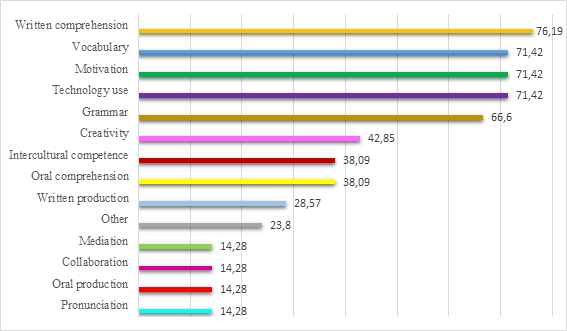
\includegraphics[width=0.9\linewidth]{image2.png}
    \source{Own elaboration (2023).}
\end{figure}

